\chapter{Trainieren des ersten Neuronale Netzes}
In dem vorherigen Kapitel haben wir gesehen,
was Maschinelles Lernen bedeutet, welche
Probleme es hilft zu lösen und warum
Deep Learning sich in der heutigen Zeit mehr und mehr durchsetzt.
Es konnte außerdem das Ziel dieser Arbeit
beschrieben und einen ersten Einblick
in die verwendete Hardware gegeben werden.
In diesem Kapitel soll es darum gehen, die
TensorFlow Bibliothek kennenzulernen
und zu zeigen wie ein Deep-Learning-Modell
für mobile Geräte (und der Google Coral Edge TPU) bereitgestellt wird.
Das Kapitel ist gegliedert nach den folgenden Schritten:
\begin{enumerate}
  \item Hole den Trainingsdatensatz.
  \item Trainiere ein neuronales Netz mit TensorFlow.
  \item Bewerte die Ergebnisse des Modells.
  \item Konvertiere das Modell in ein mobil- und TPU-kompatibles Format.
  \item Schreibe Code, um auf dem Gerät Prognosen durchzuführen.
\end{enumerate}
Die Idee dieses Kapitels stammt aus Kapitel 4 des Buchs \citetitle{book:tiny-ml}
von \textcite{book:tiny-ml} (welche involviert in der Entwicklung
der TensorFlow Lite Bibliothek sind) mit einigen
anwendungs- und hardwarespezifischen Änderungen.

\section{Das Ziel des Modells}
Ähnlich wie \autoref{sec:lernmethoden} handelt es sich
um ein einfaches Modell mit nur einer Ein- und Ausgabe.
Die zu modellierenden Daten sind etwas komplexer,
es geht um eine bekannte trigonometrische Funktion: der Sinuskurve.
Das Ziel des Modells ist es also, durch eine Eingabe $x$
den $y$-Wert $\sin(x)$ zu bestimmen.
In einer echten Anwendung könnte
diese Zahl natürlich direkt ermittelt werden,
das Beispiel soll jedoch zeigen,
wie mit Deep Learning (und sehr kleinen Netzen)
bereits anspruchsvollere, nicht lineare Daten gut modelliert werden können.
Die Sinusfunktion ist in \autoref{plot:sine-curve} zu sehen.
\begin{figure}[!h]
  \centering
  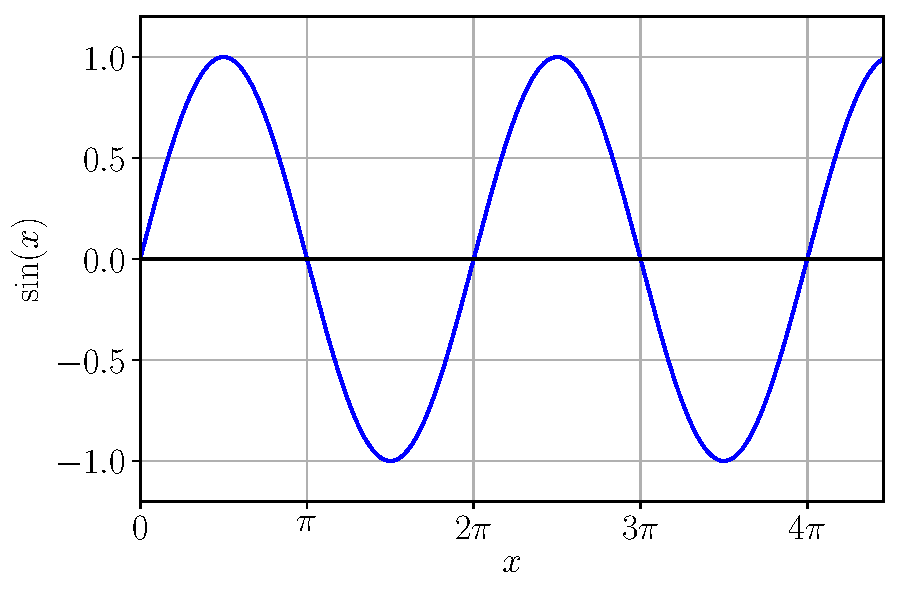
\includegraphics[width=0.7\textwidth]{first-nn/sine-curve.pdf}
  \caption{Die Sinusfunktion}
  \label{plot:sine-curve}
\end{figure}

\section{Generieren der Daten}
Neuronale Netze können komplexe Muster in den zugrundeliegenden Daten erkennen
und dabei sehr vielseitig eingesetzt werden.
In diesem Beispiel geht es wie zuvor um ein einfaches Regressionsproblem,
ein neuronales Netz kann genauso gut, aber auch für
Klassifizierung, Bildanalyse, Videoanalyse, unüberwachtes Lernen und vieles mehr verwendet werden.
Die Trainingsdaten können mit TensorFlow generiert werden und
die Vorgehensweise ist hierbei sehr ähnlich wie mit der Verwendung von NumPy:
\begin{pythoncode}
import tensorflow as tf
import math

SAMPLES = 2000

tf.random.set_seed(42)

x = tf.random.uniform((SAMPLES, 1), minval=0, maxval=2*math.pi)
tf.random.shuffle(x)

y = tf.math.sin(x)
\end{pythoncode}
Der vorhergehende Code generiert zwei Spaltenvektoren
(Trainingsdaten \pythoninline{x} und Label \pythoninline{y})
mit jeweils 2000 Werten im Bereich 0 bis $2\pi$.
Dieser Bereich nennt sich die Periode der Sinusfunktion,
da sich die Funktionswerte von dort an immer wiederholen:
\begin{figure}[!h]
  \centering
  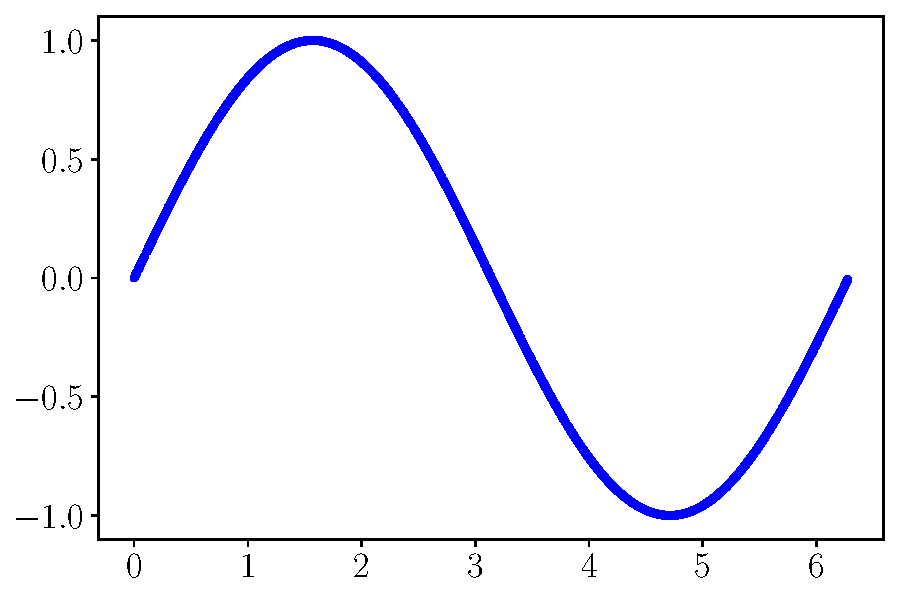
\includegraphics[width=0.7\textwidth]{first-nn/sine-data.pdf}
  \caption{Die generierten Daten}
\end{figure}

\noindent
Damit das Problem realistischer ist, wird auch für diese Daten
zufälliges Rauschen hinzugefügt:
\begin{pythoncode}
y += 0.25 * tf.random.normal(y.shape)
\end{pythoncode}
Die neuen Daten sehen wie folgt aus:
\newpage
\begin{figure}[h!]
  \centering
  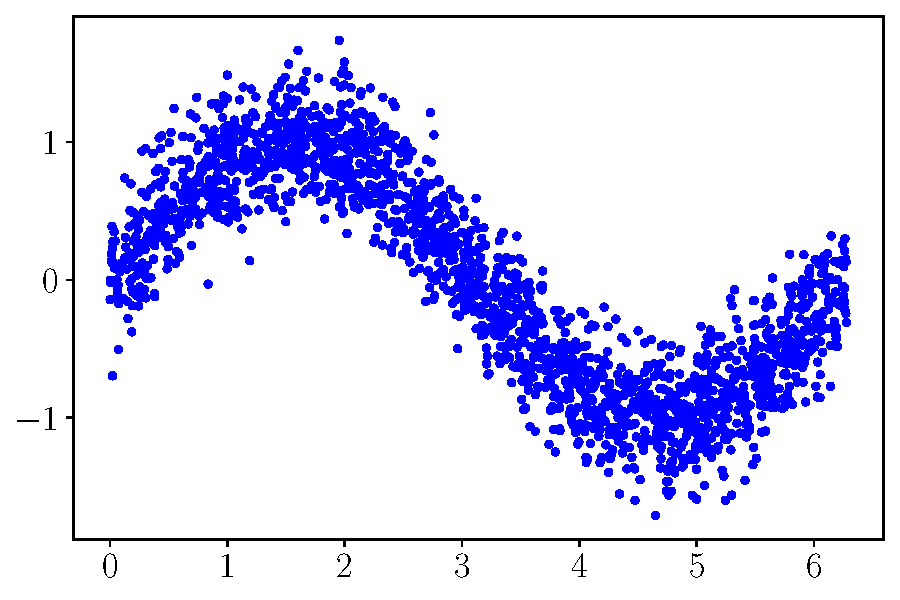
\includegraphics[width=0.7\textwidth]{first-nn/sine-data-noise.pdf}
  \caption{Die generierten Daten plus zufälliges Rauschen}
\end{figure}

\section{Aufteilen der Trainingsdaten}
Um die Qualität eines Modells bewerten zu können, werden
mehr Daten benötigt als lediglich die Trainingsbeispiele.
Dies ist der Grund warum es für gewöhnlich mehr als nur einen
Datensatz gibt. Eine typische Vorgehensweise ist die Aufgliederung
in drei Teile: dem \textit{training}, \textit{validation} und \textit{test set}.
Die Schritte, um ein passendes Modell für ein Problem zu finden, sind die Folgenden:
\begin{enumerate}
  \item Probiere verschiedene Ideen aus und trainiere einige Modelle mithilfe des
        \textit{training set}.
  \item Bewerte die Qualität der Modelle anhand des \textit{validation set} und wähle
        einen oder mehrere der vielversprechendsten Kandidaten aus.
  \item Verbessere die Leistung der ausgewählten Modelle am \textit{validation set}
        solange, bis ein Modell mit der gewünschten Qualität gefunden wurde.
        Das ausgewählte Modell kann schließlich durch das
        \textit{test set} evaluiert werden, um den Generalisierungsfehler abzuschätzen.
\end{enumerate}
Im Training sollte der Algorithmus lediglich die Trainingsdaten
zu Gesicht bekommen. Dies hilft bekannten
Fehlerquellen wie der Überanpassung (dem Gegenstück zur Unteranpassung, engl.
\textit{overfitting} und \textit{underfitting}) vorzubeugen.
Die folgende Abbildung soll die beiden Begriffe verdeutlichen.
\begin{figure}[h!]
  \centering
  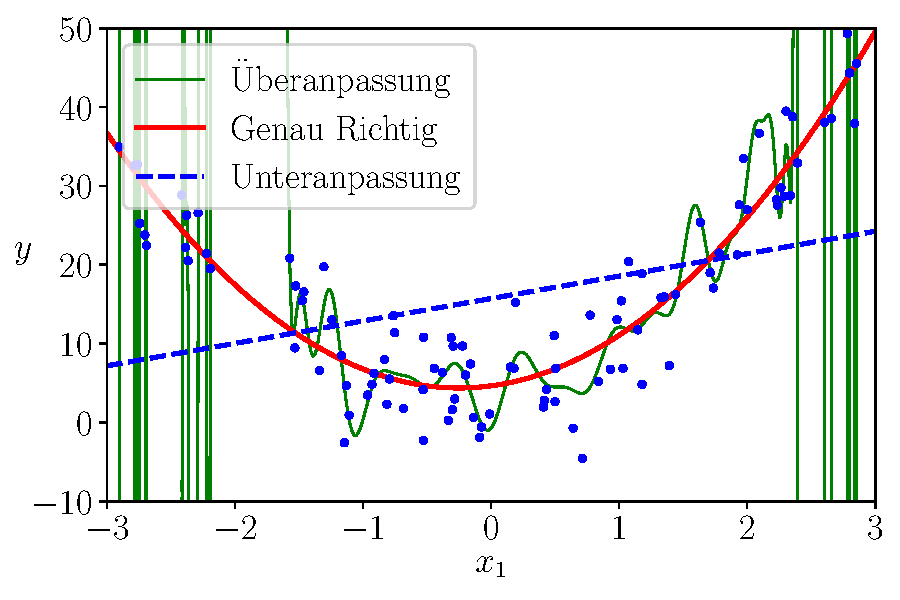
\includegraphics[width=0.7\textwidth]{first-nn/over_underfitting.pdf}
  \caption{Überanpassung und Unteranpassung am Beispiel einer
  quadratischen Funktion \parencite[131]{book:hands-on-ml}}
\end{figure}

\noindent
Modelliert ein Algorithmus die Struktur der Trainingsdaten zu gut, dann
ist die Rede von Überanpassung. Dies ist zu sehen
durch die grüne Linie. Die Funktion mag die Trainingsdaten
am besten beschreiben, schafft es aber nicht auf neue
Daten zu verallgemeinern.
Überanpassung kann erkannt werden, wenn die Leistung des Modells am
\textit{training set} steigt, während sie am \textit{validation set}
sinkt. Das Gegenstück der Überanpassung ist die
Unteranpassung. Dies zu sehen durch die blau gestreifte Linie.
Das Modell (mit nur linearen Features)
schafft es nicht die Trainingsdaten gut genug zu beschreiben.
Die besten Ergebnisse werden in diesem Beispiel durch die rote Linie erzeugt.
Um die zuvor generierten Trainingsdaten aufzuteilen,
kann die TensorFlow Methode \pythoninline{tf.split}
verwendet werden:
\begin{pythoncode}
# Wir verwenden 50% der Daten für training und 20% für testing.
# Die restlichen 30% werden für validation verwendet.
TRAIN_SIZE = int(0.5 * SAMPLES)
TEST_SIZE = int(0.2 * SAMPLES)
VAL_SIZE = SAMPLES - TRAIN_SIZE - TEST_SIZE

# Gliedere den Datensatz in drei Teile auf
x_train, x_test, x_val = tf.split(x, [TRAIN_SIZE, TEST_SIZE, VAL_SIZE])
y_train, y_test, y_val = tf.split(y, [TRAIN_SIZE, TEST_SIZE, VAL_SIZE])

# Verifiziere die Aufteilung, durch summieren der Größen
assert tf.size(x_train) + tf.size(x_test) + tf.size(x_val) == SAMPLES
\end{pythoncode}
Die drei Datensätze können nun in der folgenden Abbildung farblich dargestellt werden.
\begin{figure}[h!]
  \centering
  \includegraphics[width=0.7\textwidth]{first-nn/sine-data-noise-legend.pdf}
  \caption{Aufteilung der Sinusdaten in
  \textit{training}, \textit{validation} und \textit{test set}}
\end{figure}

\section{Definieren eines grundlegenden Modells}
Ein neuronales Netz besteht aus mehreren kleinen Einheiten (auch Neuronen genannt).
Jedes Neuron nimmt entgegen ein bis $n$ numerische Eingaben, führt einige
einfache Berechnungen durch und produziert eine numerische Ausgabe.
Alleine kann ein Neuron kaum die einfachsten Probleme lösen, doch zusammen
durch Komposition und Training haben sie das Potenzial,
die komplexe Welt verstehen.
Der Aufbau eines einzelnen Neuron ist in \autoref{fig:nn-neuron} zu sehen.
\newpage
\begin{figure}[h!]
  \centering
  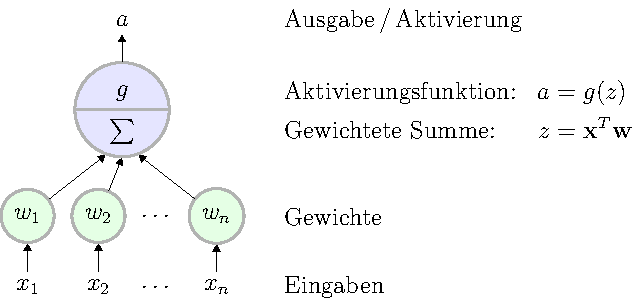
\includegraphics{first-nn/nn-neuron.pdf}
  \caption{Der Aufbau eines einzelnen Neuron}
  \label{fig:nn-neuron}
\end{figure}
\noindent
Als erster Schritt wird eine gewichtete Summe
($z = w_1x_1 + w_2x_2 +\dotsb+ w_nx_n = \mathbf{x}^T\mathbf{w}$)
der Eingabewerte berechnet. Die Elemente $\mathbf{x}$ und $\mathbf{w}$
sind Spaltenvektoren der Form: $(x_1,\dotsc,x_n)^T$ und $(w_1,\dotsc,w_n)^T$.
\footnote{Wie immer wird versucht Berechnungen als Vektor- und Matrixoperationen
auszudrücken um CPU und GPU Beschleunigung auszunutzen.}
Der zweite Schritt wendet eine Aktivierungsfunktion an und dies
erzeugt die Ausgabe: $y = a(z)$. Ein neuronales Netz
besteht aus der Verknüpfung verschiedener Neuronen und die
Gewichte stellen die erlernbaren Parameter dar.
\autoref{fig:example-nn} zeigt ein einfaches neuronales Netz
mit zwei verdeckten Schichten (engl. \textit{hidden layers}).
\begin{figure}[h!]
  \centering
  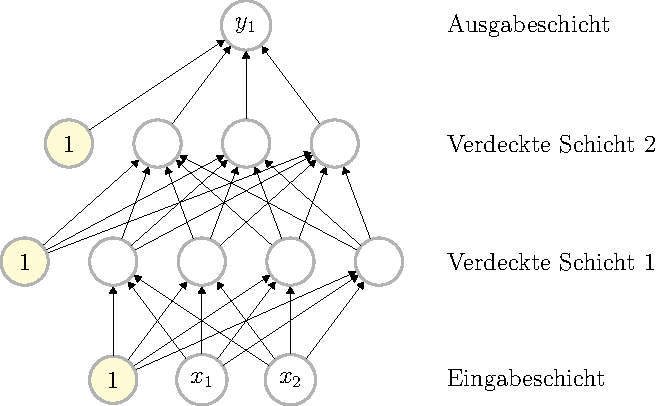
\includegraphics{first-nn/example-nn.pdf}
  \caption{Ein einfaches neuronales Netz mit zwei verdeckten Schichten}
  \label{fig:example-nn}
\end{figure}
\noindent
Verdeckte Schichten sind all diejenigen, die nicht Ein- oder Ausgabe sind.
Jede Schicht außer der Ausgabeschicht enthält ein Bias-Neuron
(in Gelb markiert), welches immer Eins ausgibt, aber auch trainiert werden kann
und ist vollständig mit der nächsten Schicht verbunden.
Ein neuronales Netz wird tief genannt, wenn es viele verdeckte Schichten besitzt.
\footnote{In den 1990er-Jahren wurde ein neuronales Netz
mit mehr als zwei verdeckten Schichten als tief angesehen.
Da es aber heutzutage Netze mit Dutzend und Hunderten von Schichten
gibt, ist die Definition von \enquote{tief} etwas schwammig \parencite[289]{book:hands-on-ml}.}
Ein neuronales Netz wird durch einen Algorithmus trainiert, der
sich Backpropagation nennt.